\chapter{Présentation Général de l’IOT} \label{chap:Présentation général de l’IOT}
\section{Définition de IOT}
L'Internet des objets (IdO) est un système d'appareils informatiques interconnectés, de machines mécaniques et numériques, d'objets, d'animaux ou de personnes avec des identifiants uniques (UID) qui nécessitent une communication inter-humaine. Interaction humaine Nécessite une connexion humaine. Interaction homme ou homme-ordinateur.[10] ses fondamentaux caractéristiques sont comme shivalibhadaniya écrit  [11]: \newline
Connectivité \newline
La connectivité est une exigence importante de l’infrastructure IoT. Les objets de l’IoT doivent être connectés à l’infrastructure IoT. N’importe qui, n’importe où, n’importe quand peut se connecter, cela devrait être garanti à tout moment. Par exemple, la connexion entre les personnes via des appareils Internet tels que les téléphones mobiles et d’autres gadgets, ainsi que la connexion entre les appareils Internet tels que les routeurs, les passerelles, les capteurs, etc.  \newline                            
Intelligence et identité \newline
L’extraction de connaissances à partir des données générées est très importante. Par exemple, un capteur génère des données, mais ces données ne seront utiles que si elles sont correctement interprétées. Chaque appareil IoT a une identité unique. Cette identification est utile pour suivre l’équipement et parfois pour interroger son état.\newline
 
Évolutivité \newline
Le nombre d’éléments connectés à la zone IoT augmente de jour en jour. Par conséquent, une configuration IoT devrait être capable de gérer l’expansion massive. Les données générées en tant que résultat sont énormes et doivent être traitées de manière appropriée.\newline
 
Dynamique et auto-adaptatif (complexité) \newline
 Les appareils IoT doivent s’adapter de manière dynamique aux contextes et scénarios changeants. Supposons une caméra destinée à la surveillance. Il doit être adaptable pour travailler dans différentes conditions et différentes situations d’éclairage (matin, après-midi, nuit).\newline
 
Architecture \newline
l’architecture IoT ne peut pas être de nature homogène. Il doit être hybride, prenant en charge les produits de différents fabricants pour fonctionner dans le réseau IoT. IoT n’appartient à aucune branche d’ingénierie. L’IoT est une réalité lorsque plusieurs domaines se rejoignent.\newline
 
Sécurité \newline
Il existe un risque que les données personnelles sensibles des utilisateurs soient compromises lorsque tous leurs appareils sont connectés à Internet. Cela peut entraîner une perte pour l’utilisateur. La sécurité des données est donc le défi majeur. De plus, l’équipement impliqué est énorme. Les réseaux IoT peuvent également être à risque. Par conséquent, la sécurité des équipements est également essentielle.
\section{Les Capteurs}
 Les capteurs de l'Internet des objets (IoT) sont des capteurs qui collectent des données environnementales et les envoient à un réseau pour traitement. Ils font partie d'un système en réseau qui peut être utilisé pour surveiller, contrôler et automatiser les processus dans divers domaines. Voici les capteurs qui sont nous soucions :
\subsection{Capteur d'humidité température numérique DHT22}
Le capteur numérique d'humidité et de température DHT22 est un capteur capacitif qui peut mesurer simultanément la température de l'air ambiant et l'humidité relative. 
\begin{figure}[hbt]
\centering
\label{fig:Capteur DHT22}


 \fcolorbox{black}{white}{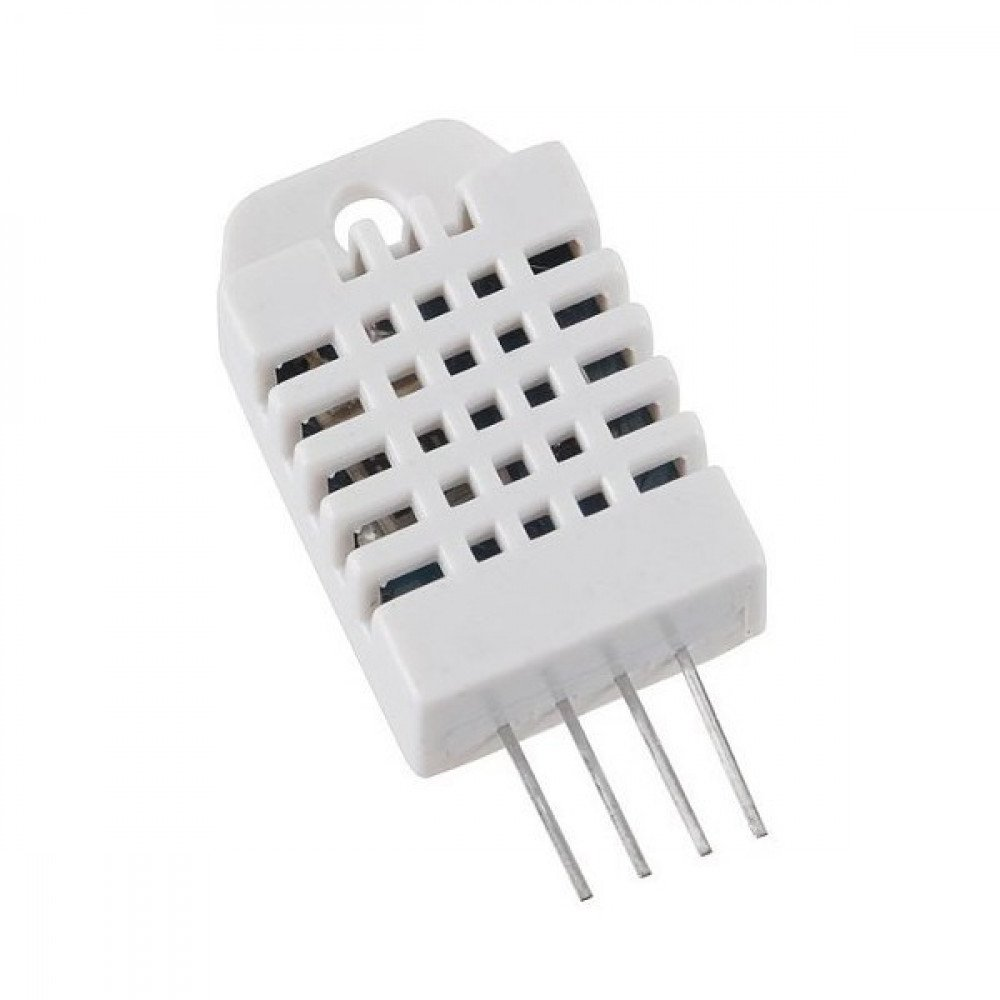
\includegraphics[width=6cm]{figures/DZD001646_2-1000x1000.jpg}}
 \caption{Capteur DHT22 [12]}
\end{figure}
\subsection{Capteur de Lumière TSL2561}
Le capteur de lumière TSL2561 est un capteur de lumière ambiante numérique qui mesure la lumière visible et infrarouge pour fournir des données précises sur la luminosité ambiante

\begin{figure}[hbt]
\centering
\label{fig:Capteur TSL2561}


 \fcolorbox{black}{white}{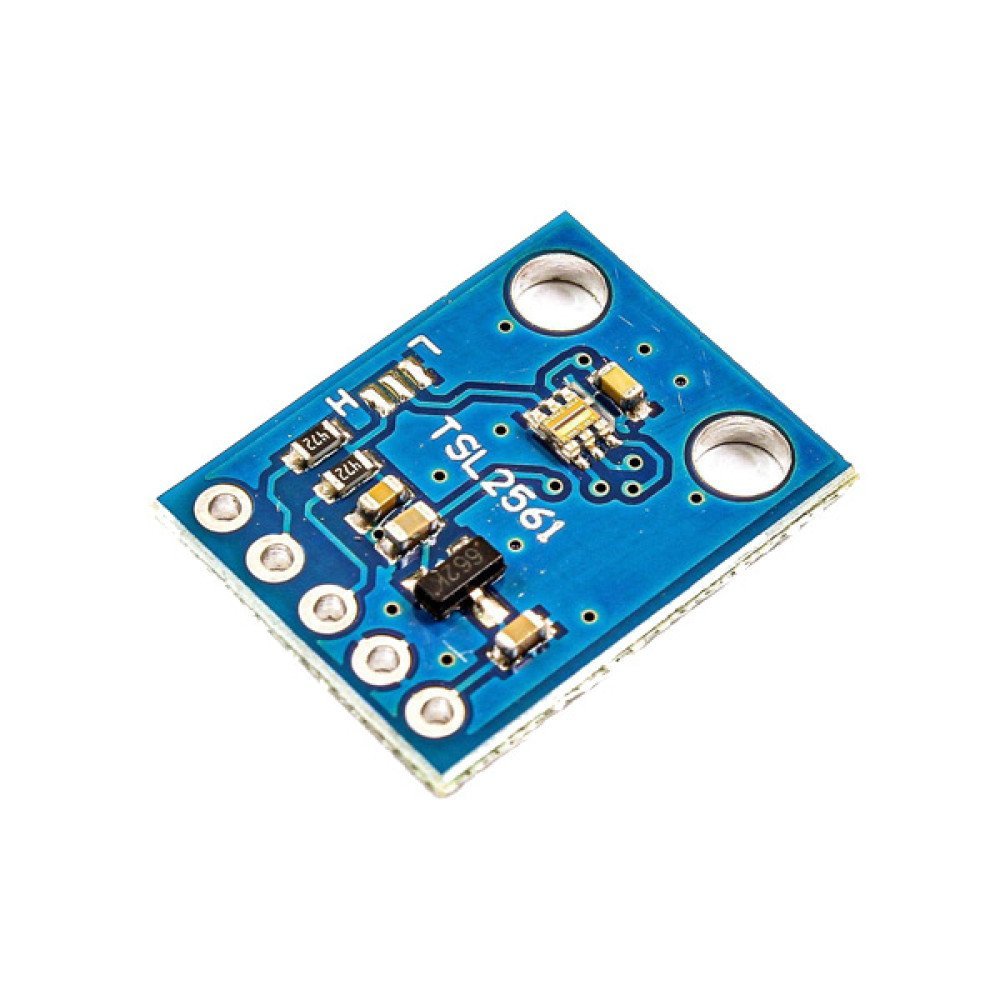
\includegraphics[width=6cm]{figures/DZD005019_1-1000x1000.jpeg}}
 \caption{Capteur TSL2561 [13]}
\end{figure}

\subsection{Capteur d'humidité du sol FC-28}
Le capteur d'humidité du sol FC-28 est un capteur analogique pour mesurer l'humidité du sol. Il est souvent utilisé dans des applications telles que l'agriculture et l'irrigation automatique
\begin{figure}[hbt]
\centering
\label{fig:Capteur FC-28}

\fcolorbox{black}{white}{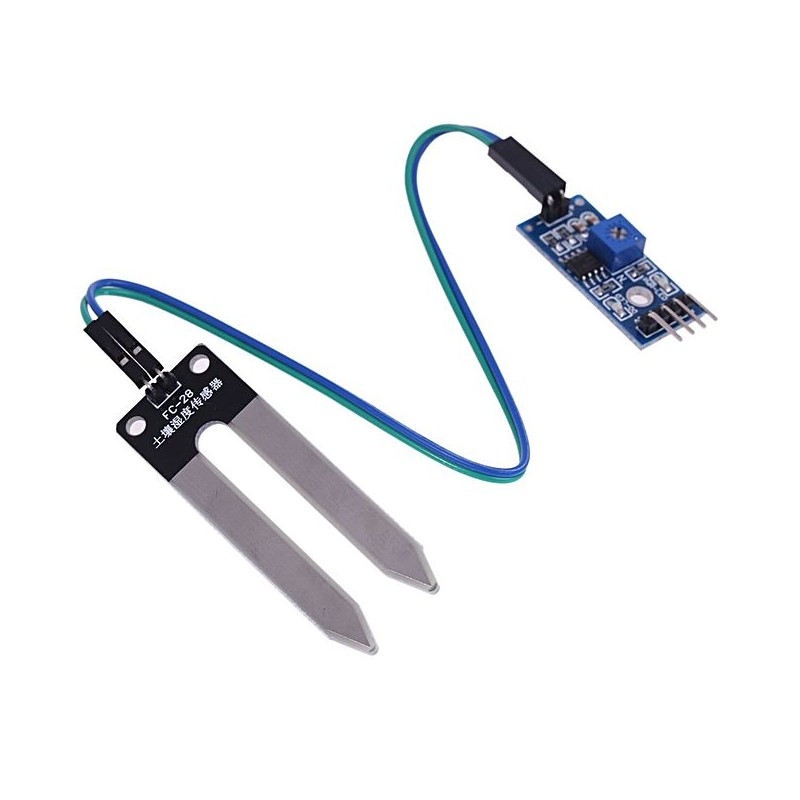
\includegraphics[width=6.5cm,frame]{figures/arduino-capteur-d-humidite-du-sol-pour-arduino.jpg}}
\caption{Capteur FC-28 [14]}
\end{figure}

\section{Micro-contrôleur Arduino Uno}
Un micro-contrôleur Arduino est une carte électronique basée sur un micro-contrôleur qui peut être programmée pour contrôler diverses tâches . Les micro-contrôleurs Arduino se composent généralement d'un processeur, d'une mémoire, d'entrées et de sorties numériques et analogiques et de circuits supplémentaires pour la communication et la programmation.  
\begin{figure}[hbt]
\centering
\label{fig:Arduino Uno}

 \fcolorbox{black}{white} {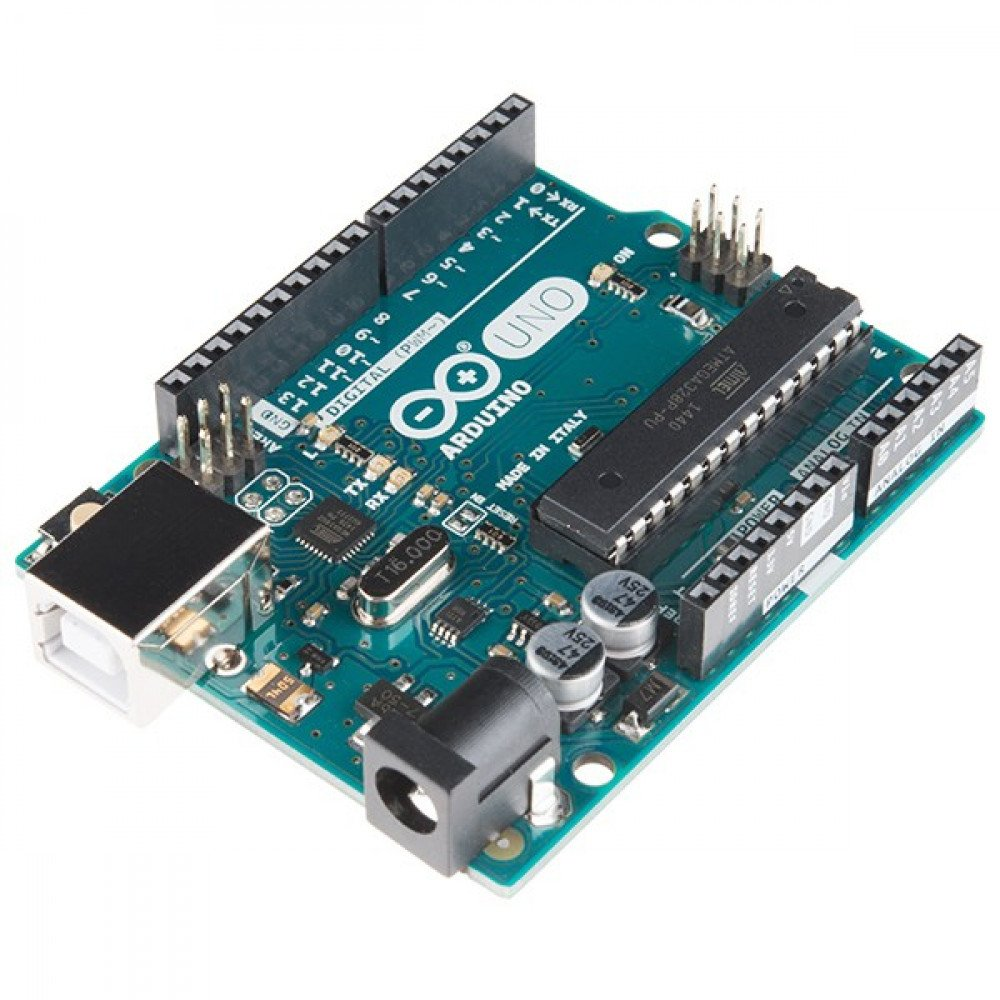
\includegraphics[width=10cm]{figures/DZD000371-1000x1000.jpg}}
  \caption{Arduino Uno [15]}
\end{figure}
\pagebreak
\section{Relais}

Le relais est un composant électromécanique qui permet d'ouvrir ou fermer un contacteur et est un déclencheur de bas niveau 5V.que sera relais directement avec un Arduino d’un cote et de contacteur de l’autre cote . Comme c’est il n’y a pas des ventilateur de serres et électrovanne intelligentes et l’Arduino n’est pas compatible de déclencher des dispositifs de grands voltages d’électricité nous avants besoin de relais. 
\begin{figure}[hbt]
\centering
\label{fig:Déclencheur 5V}

 \fcolorbox{black}{white}{ 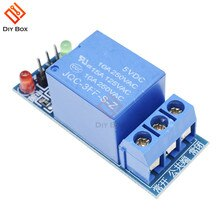
\includegraphics[width=6cm]{figures/D-clencheur-de-bas-niveau-5V-Module-de-relais-1-canal-bouclier-d-interface-cc-220V.jpg_220x220.jpg}}
  \caption{Déclencheur 5V[16]}
\end{figure}
\section{Contacteur BE101 NP2}
Un contacteur est un appareil électrotechnique destiné à établir ou interrompre le passage du courant, à partir d'une commande à distance,Il a la même fonction qu'un relais électromécanique, sauf que ses contacts sont prévus pour supporter un courant beaucoup plus important
\begin{figure}[hbt]
\centering
\label{Contacteur BE101 NP2}
  \fcolorbox{black}{white}{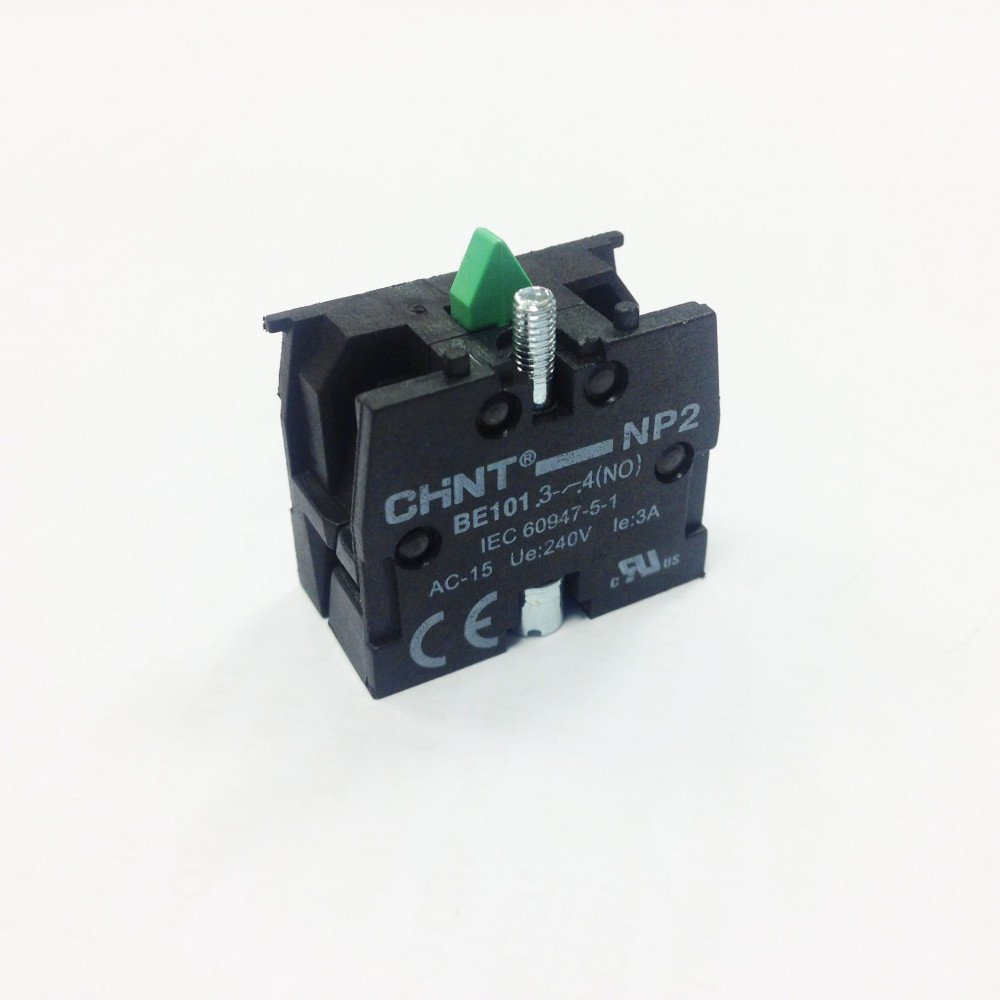
\includegraphics[width=5cm]{figures/DZD002759_1-1000x1000h.JPG}}
  \caption{Contacteur BE101 NP2 [17]}
\end{figure}
 \section{Unité de commande}
 Dans notre système proposé est  équipée d'un micro-contrôleur Arduino Uno , d'une connectivité réseau sans fil avec les capteurs , d'une mémoire pour stocker les données « application».
Les unités de commande IoT peuvent être programmées pour surveiller en temps réel les données des capteurs, déclencher des actions en réponse à des événements, envoyer des alertes en cas de situations anormales et collecter des données pour l'analyse et la prise de décision soi localement ou niveau de l’Arduino ou bien dans le serveur.
\section{Conclusion}
Dans le contenu précédant  nous avons précise tous qui est nous concernons dans notre système proposée et disponible dans le marche algérien , ce matériel nous aide a collecte les données en temps réel et les stockeras dans une base de données.   

 

